% Simplified pipeline of the class-conditional DDPM with classifier-free guidance.
% Build:  pdflatex pipeline.tex   (or: tectonic pipeline.tex)
\documentclass[tikz,border=8pt]{standalone}
\usepackage{amsmath,amssymb}
\usepackage[T1]{fontenc}
\usepackage{lmodern}
\usetikzlibrary{positioning,arrows.meta,fit,backgrounds}

\definecolor{cData}{HTML}{3B6EA8}
\definecolor{cOp}{HTML}{C77C1E}
\definecolor{cNet}{HTML}{3A8A55}
\definecolor{cLoss}{HTML}{B5443B}

\tikzset{
  >={Stealth[length=2.4mm]},
  node distance=10mm,
  box/.style={draw, rounded corners=4pt, align=center, minimum height=15mm, minimum width=34mm,
              inner sep=5pt, line width=0.8pt},
  data/.style={box, draw=cData, fill=cData!8},
  op/.style={box, draw=cOp, fill=cOp!9},
  net/.style={box, draw=cNet, fill=cNet!10},
  loss/.style={box, draw=cLoss, fill=cLoss!8},
  arr/.style={->, line width=0.9pt},
  lbl/.style={font=\footnotesize, inner sep=2pt},
  panel/.style={draw=gray!55, rounded corners=8pt, dashed, line width=0.6pt, inner sep=8pt},
  ptitle/.style={font=\bfseries, anchor=south west, inner sep=2pt},
}

\begin{document}
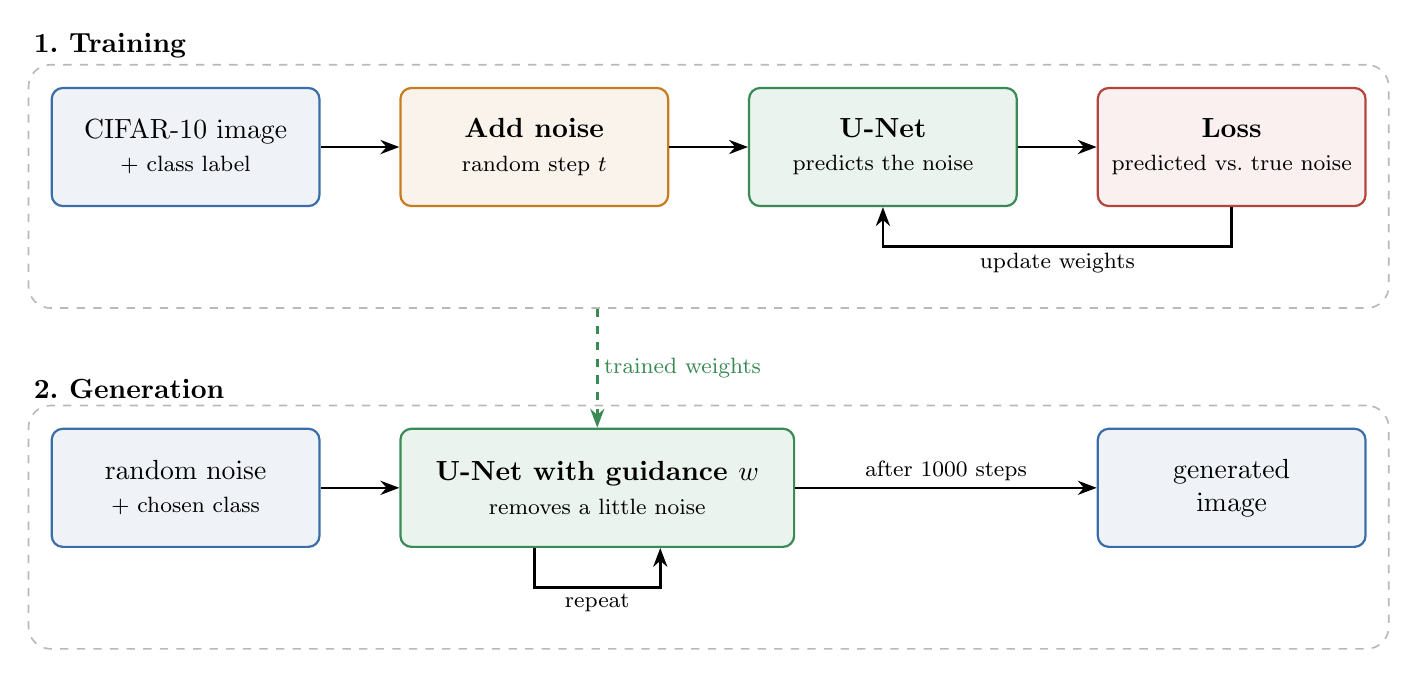
\begin{tikzpicture}

% ---------------- Training ----------------
\node[data] (img) {CIFAR-10 image\\ \footnotesize + class label};
\node[op, right=of img] (noise) {\textbf{Add noise}\\ \footnotesize random step $t$};
\node[net, right=of noise] (unet) {\textbf{U-Net}\\ \footnotesize predicts the noise};
\node[loss, right=of unet] (loss) {\textbf{Loss}\\ \footnotesize predicted vs.\ true noise};

\draw[arr] (img) -- (noise);
\draw[arr] (noise) -- (unet);
\draw[arr] (unet) -- (loss);
\draw[arr] (loss.south) -- ++(0,-5mm) -| node[lbl, pos=0.25, below] {update weights} (unet.south);

\begin{scope}[on background layer]
  \node[panel, fit={(img)(loss)([yshift=-10mm]loss.south)}] (pA) {};
\end{scope}
\node[ptitle] at (pA.north west) {1.\ Training};

% ---------------- Generation ----------------
\node[data, below=28mm of img] (z) {random noise\\ \footnotesize + chosen class};
\node[net, right=of z, minimum width=50mm] (cfg)
  {\textbf{U-Net with guidance $w$}\\ \footnotesize removes a little noise};
\node[data] (out) at (loss |- z) {generated\\ image};

\draw[arr] (z) -- (cfg);
\draw[arr] (cfg) -- node[lbl, above] {after 1000 steps} (out);
\draw[arr] (cfg.south) ++(-8mm,0) -- ++(0,-5mm) -- ++(16mm,0) node[lbl, below, midway] {repeat} -- ++(0,5mm);

\begin{scope}[on background layer]
  \node[panel, fit={(z)(out)(cfg)([yshift=-10mm]cfg.south)}] (pB) {};
\end{scope}
\node[ptitle] at (pB.north west) {2.\ Generation};

\draw[arr, dashed, cNet] (cfg.north |- pA.south) -- node[lbl, right, text=cNet] {trained weights} (cfg.north);

\end{tikzpicture}
\end{document}
